\documentclass{article}
\usepackage[T1]{fontenc}
\usepackage{helvet}
\usepackage{listings}
\usepackage[utf8]{inputenc}
\usepackage[english]{babel}
\usepackage{booktabs} 
\usepackage{longtable} 
\usepackage{xcolor}
\usepackage{setspace}
\usepackage{subcaption}
\usepackage[letterpaper,top=2cm,bottom=2cm,left=3cm,right=3cm,marginparwidth=1.75cm]{geometry}
\usepackage{xstring}
\usepackage{amsmath}
\usepackage{amssymb}
\usepackage{graphicx}
\usepackage[labelfont=sf,textfont=it,font=small]{caption}
\usepackage{authblk}
\usepackage[colorlinks=true, allcolors=blue]{hyperref}
\usepackage[authoryear,round]{natbib}  
\usepackage{titlesec}

\renewcommand{\familydefault}{\sfdefault}
\newcommand{\orcidlink}[1]{} 

\onehalfspacing 
\setlength{\parskip}{0.5em}

\titleformat{\section}
  {\normalfont\Large\bfseries\scshape}{\thesection}{1em}{}
\titleformat{name=\section,numberless}
  {\normalfont\Large\bfseries\scshape}{}{0em}{}
\titleformat{\subsection}
  {\normalfont\large\bfseries\scshape}{\thesubsection}{1em}{}
\titleformat{\subsubsection}
  {\normalfont\normalsize\bfseries\scshape}{\thesubsubsection}{1em}{}



\author[1,*]{Mattia Bruscia\,\orcidlink{0000-0003-0910-6445}}
\author[1]{William Nardin\,\orcidlink{0000-0002-5490-879X}}
\author[1]{Xiaoxu Guo}
\author[1]{Limin Sun}
\author[2]{Giulia Franchi}

\affil[1]{University of Maryland Center for Environmental Science (UMCES), Horn Point Laboratory, 2020 Horns Point Road, Cambridge, MD 21613, USA}
\affil[2]{Department of Computer Science, Salisbury University, 1101 Camden Avenue, Salisbury, MD 21801, USA}

\affil[ ]{\textit{Author emails}: mbruscia@umces.edu (MB), wnardin@umces.edu (WN), xguo@umces.edu (XG), lmsun@umces.edu (LS), franchigiulia2025@gmail.com (GF)}

\affil[ ]{\textit{Corresponding author}: *mbruscia@umces.edu}

\date{} 

\title{Multiscale Feature Extraction with Wavelet Scattering Transform for Remote Sensing Vegetation Classification via Machine Learning}

\begin{document}
\maketitle

\begin{center}
\textbf{\textsc{Abstract}}
\end{center}

Land cover classification via Machine Learning is essential for ecological monitoring, but its reliability is often compromised by noisy imagery and limited datasets, common challenges in UAV acquisitions. Adopting advanced feature extraction is crucial to maintain accuracy under suboptimal conditions. This study evaluates the Wavelet Scattering Transform (WST) as a feature extraction technique for Random Forest-based classification across three coastal sites in the Chesapeake Bay region (Maryland, USA) representing diverse ecological environments.

The experimental framework comprised $1512$ classification experiments spanning six noise types, three dataset sizes (5–40 images per class), and three feature extraction methods: advanced statistical descriptors, WST, and a hybrid approach combining both.

Key findings demonstrate that the Hybrid method achieves statistically significant improvements over the statistical baseline. The Hybrid approach exhibits superior noise robustness, degrading slower than Advanced Statistics. Under extreme data scarcity, all methods retain strong data efficiency.
However, WST alone does not significantly outperform traditional statistical features, and its substantial computational overhead is not justified in low-noise conditions. These results provide practical guidance for UAV-based monitoring: Hybrid features are recommended for high-noise scenarios with GPU acceleration, while simpler statistical approaches suffice for clean imagery or resource-constrained deployments.

\textbf{\textsc{Keywords}}
Feature extraction, Wavelet Scattering Transform, Vegetation Classification, Ecological Restoration, Wetland Monitoring, UAV Remote Sensing, Machine Learning, Drones

\section{Introduction}

Coastal wetlands—including salt marshes, mangroves, and estuaries—are among the most productive ecosystems on Earth. They provide critical services such as carbon sequestration, pollutant filtration, and protection against storm surges \cite{zedler2005wetland, barbier2011value, Mitsch2013}, while supporting global fisheries and tourism. Despite their value, these ecosystems face unprecedented threats from urbanization, pollution, and climate change, manifesting through rising sea levels and extreme weather events \cite{worm2006impacts}. Eutrophication and erosion further destabilize these habitats, with salt marshes being particularly vulnerable. Recent studies indicate that marsh sediments also accumulate microplastics, serving as indicators of anthropogenic pressure \cite{lloret2020microplastics}.

Given these threats, effective monitoring is a critical priority. Traditional field methods are labor-intensive and impractical for large areas \cite{Xue2017Significant}. Remote sensing, particularly Unmanned Aerial Vehicles (UAVs), has emerged as a powerful alternative, enabling efficient data collection over complex landscapes \cite{Zhang2016Remote}. UAVs offer sub-centimeter resolution, flexibility, and multisensor integration, making them essential for vegetation mapping and biomass estimation \cite{Ma, Correll2019, nardin2020ndvi, wan2014spartina, doughty2019mapping, adade2021uav}. Long-term monitoring in the Chesapeake Bay exemplifies UAV application across diverse environments: Poplar Island (restored via dredged sediment), Assateague Island (natural barrier island), and Sunset Island (managed `living shoreline'). These sites exhibit complex morphological changes driven by erosion and sea level rise, underscoring the urgency for scalable, automated monitoring methodologies \cite{VALIELA20181148}.

While promising, UAV imagery is susceptible to degradation from sensor noise, motion blur, and environmental factors, which limit classification accuracy. Furthermore, ecological restoration sites often lack the extensive labeled datasets required for supervised learning. Traditional feature extraction (e.g., statistical descriptors) is interpretable but often lacks robustness to noise and complex spatial patterns. Conversely, Convolutional Neural Networks (CNNs), while effective, require large training corpora—often unavailable in ecological contexts—and function as black-box models, limiting interpretability regarding feature importance.

This study addresses these challenges by investigating the Wavelet Scattering Transform (WST) for robust land cover classification under noisy and data-scarce conditions. The WST computes multi-scale, invariant representations through iterative wavelet decompositions \cite{Mallat2012, Bruna2013Invariant}, capturing hierarchical patterns without the training requirements of deep learning. The novelty of this work lies in a systematic evaluation of WST performance across six noise types and three dataset sizes, benchmarking it against statistical and hybrid (WST + statistical) approaches using a Random Forest classifier. Rigorous statistical validation, including Wilcoxon signed-rank tests and Cohen's $d$, supports the analysis of UAV imagery from Poplar, Assateague, and Sunset Islands. Our findings demonstrate WST's superior robustness under high noise (e.g., Gaussian $\sigma=50$, Speckle variance=55). The hybrid approach yields statistically significant improvements in Macro-F1 score ($p=0.039$, Cohen's $d=0.156$) over baselines, although the computational cost of WST is less justified under clean conditions.

The paper is organized as follows. Section 1 introduces the research context. Section 2 details the experimental framework, including study areas, data acquisition, and the methodological pipeline. Section 3 presents quantitative results across noise conditions and dataset sizes. Finally, Section 4 discusses findings, methodological limitations, and implications for operational wetland monitoring.

\section{Materials and Methods}

\subsection{Study Sites}

The study focused on three coastal sites in Maryland (USA), within the Chesapeake Bay area, selected to represent diverse ecological settings and anthropogenic impacts. Figure~\ref{fig:siti} shows representative aerial views of these locations, where the dominant plant species is *Spartina alterniflora*.

Poplar Island (38°46'N, 76°23'W) is an artificial island undergoing a major restoration initiative, the Paul S. Sarbanes Ecosystem Restoration Project. Measuring approximately 5.6 km by 0.8 km, it was reconstructed using dredged sediments from Baltimore navigation channels. Jointly managed by the USACE and MDOT MPA, the project aims to restore 694 hectares of tidal wetland and terrestrial habitat. The island is organized into diked containment cells for sediment management, designed to eventually support equal portions of marsh and terrestrial zones.

Assateague Island (38°14'N, 75°09'W), a barrier island extending over 60 km, is managed primarily by the National Park Service and U.S. Fish and Wildlife Service. It features areas characterized by natural coastal dynamics alongside sections with shoreline interventions intended to mitigate erosion. Hosting extensive dunes, maritime forests, and salt marshes, the island provides a valuable comparison between natural and intensively managed coastal environments.

Sunset Island (38°19'N, 75°05'W) is a managed environment in Isle of Wight Bay, near Ocean City. It serves as an ecological laboratory for a `living shoreline' project designed to stabilize the waterfront while enhancing habitat diversity. Characterized by a blend of urban waterfronts and restored features, it exemplifies the integration of ecological restoration within urbanized settings. Its inclusion provides a crucial benchmark for evaluating nature-based engineering solutions against more natural coastal systems.

\begin{figure}[t]
    \centering
    
    % --- Prima riga: (a) e (b) ---
    % Allineamento [b] per le didascalie
    \begin{minipage}[b]{0.45\textwidth}
        \centering
        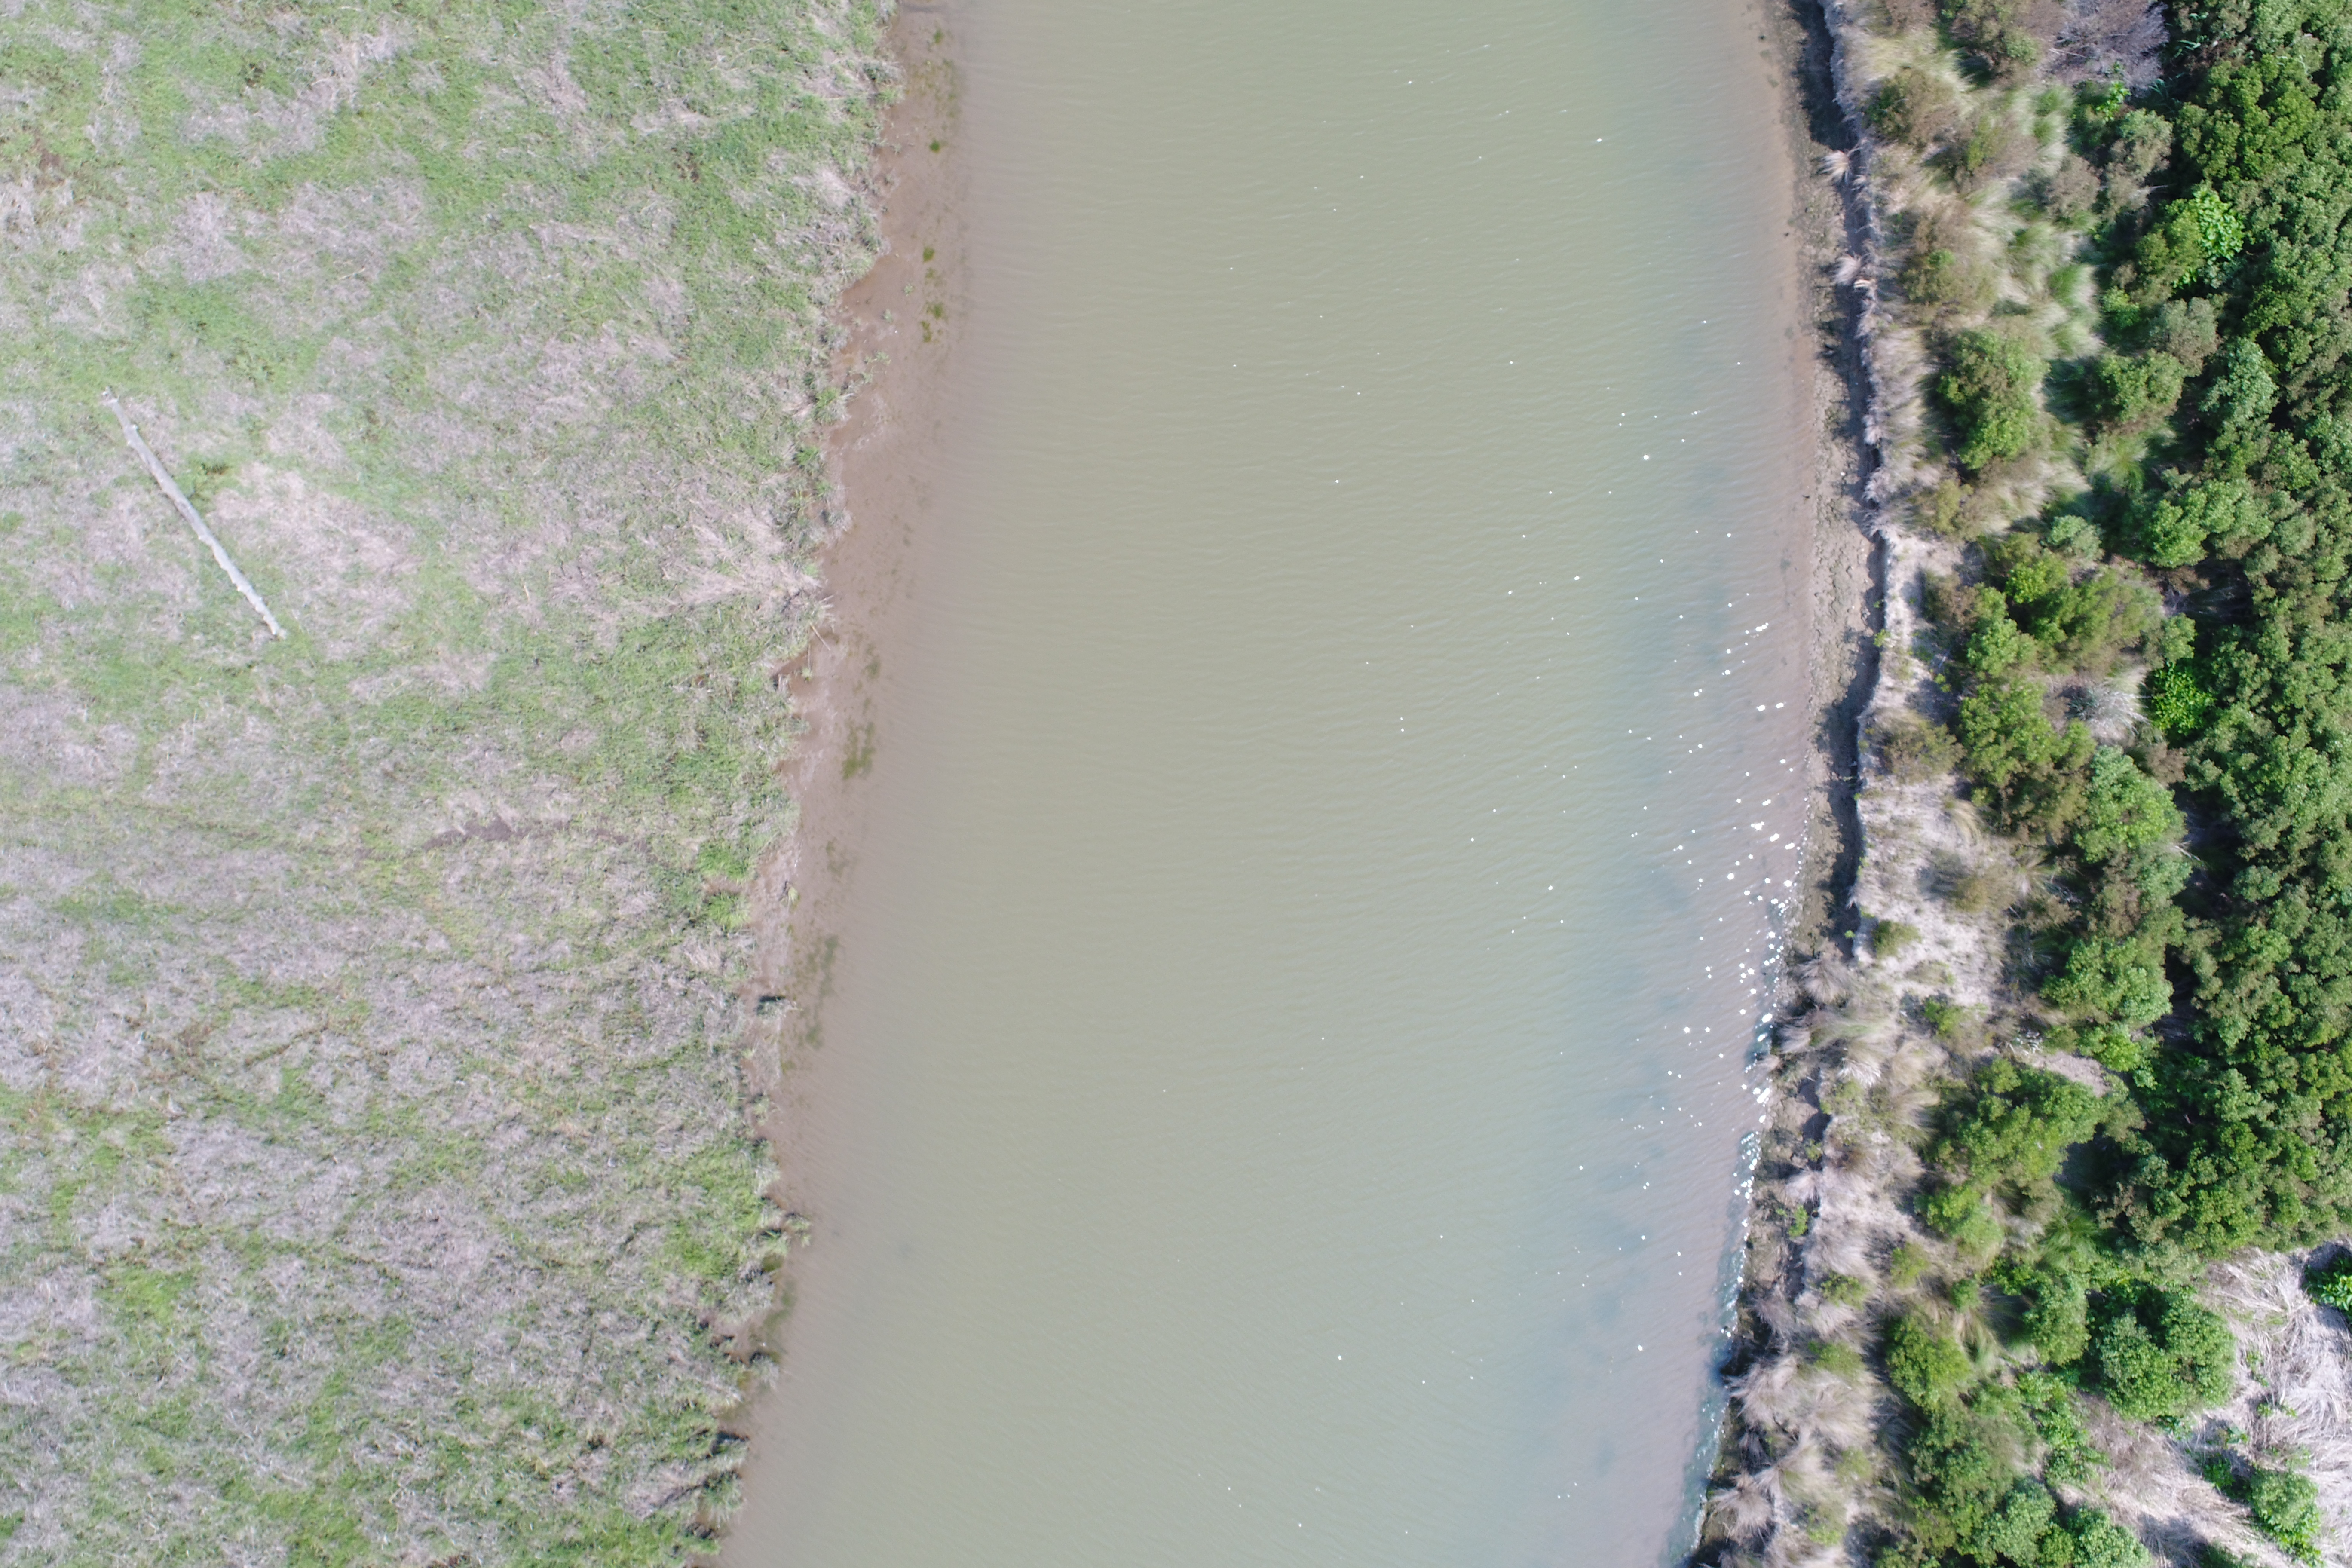
\includegraphics[width=\textwidth]{images/site_poplar_island_aerial.JPG} \\
        (a)
    \end{minipage}
    \hfill
    \begin{minipage}[b]{0.45\textwidth}
        \centering
        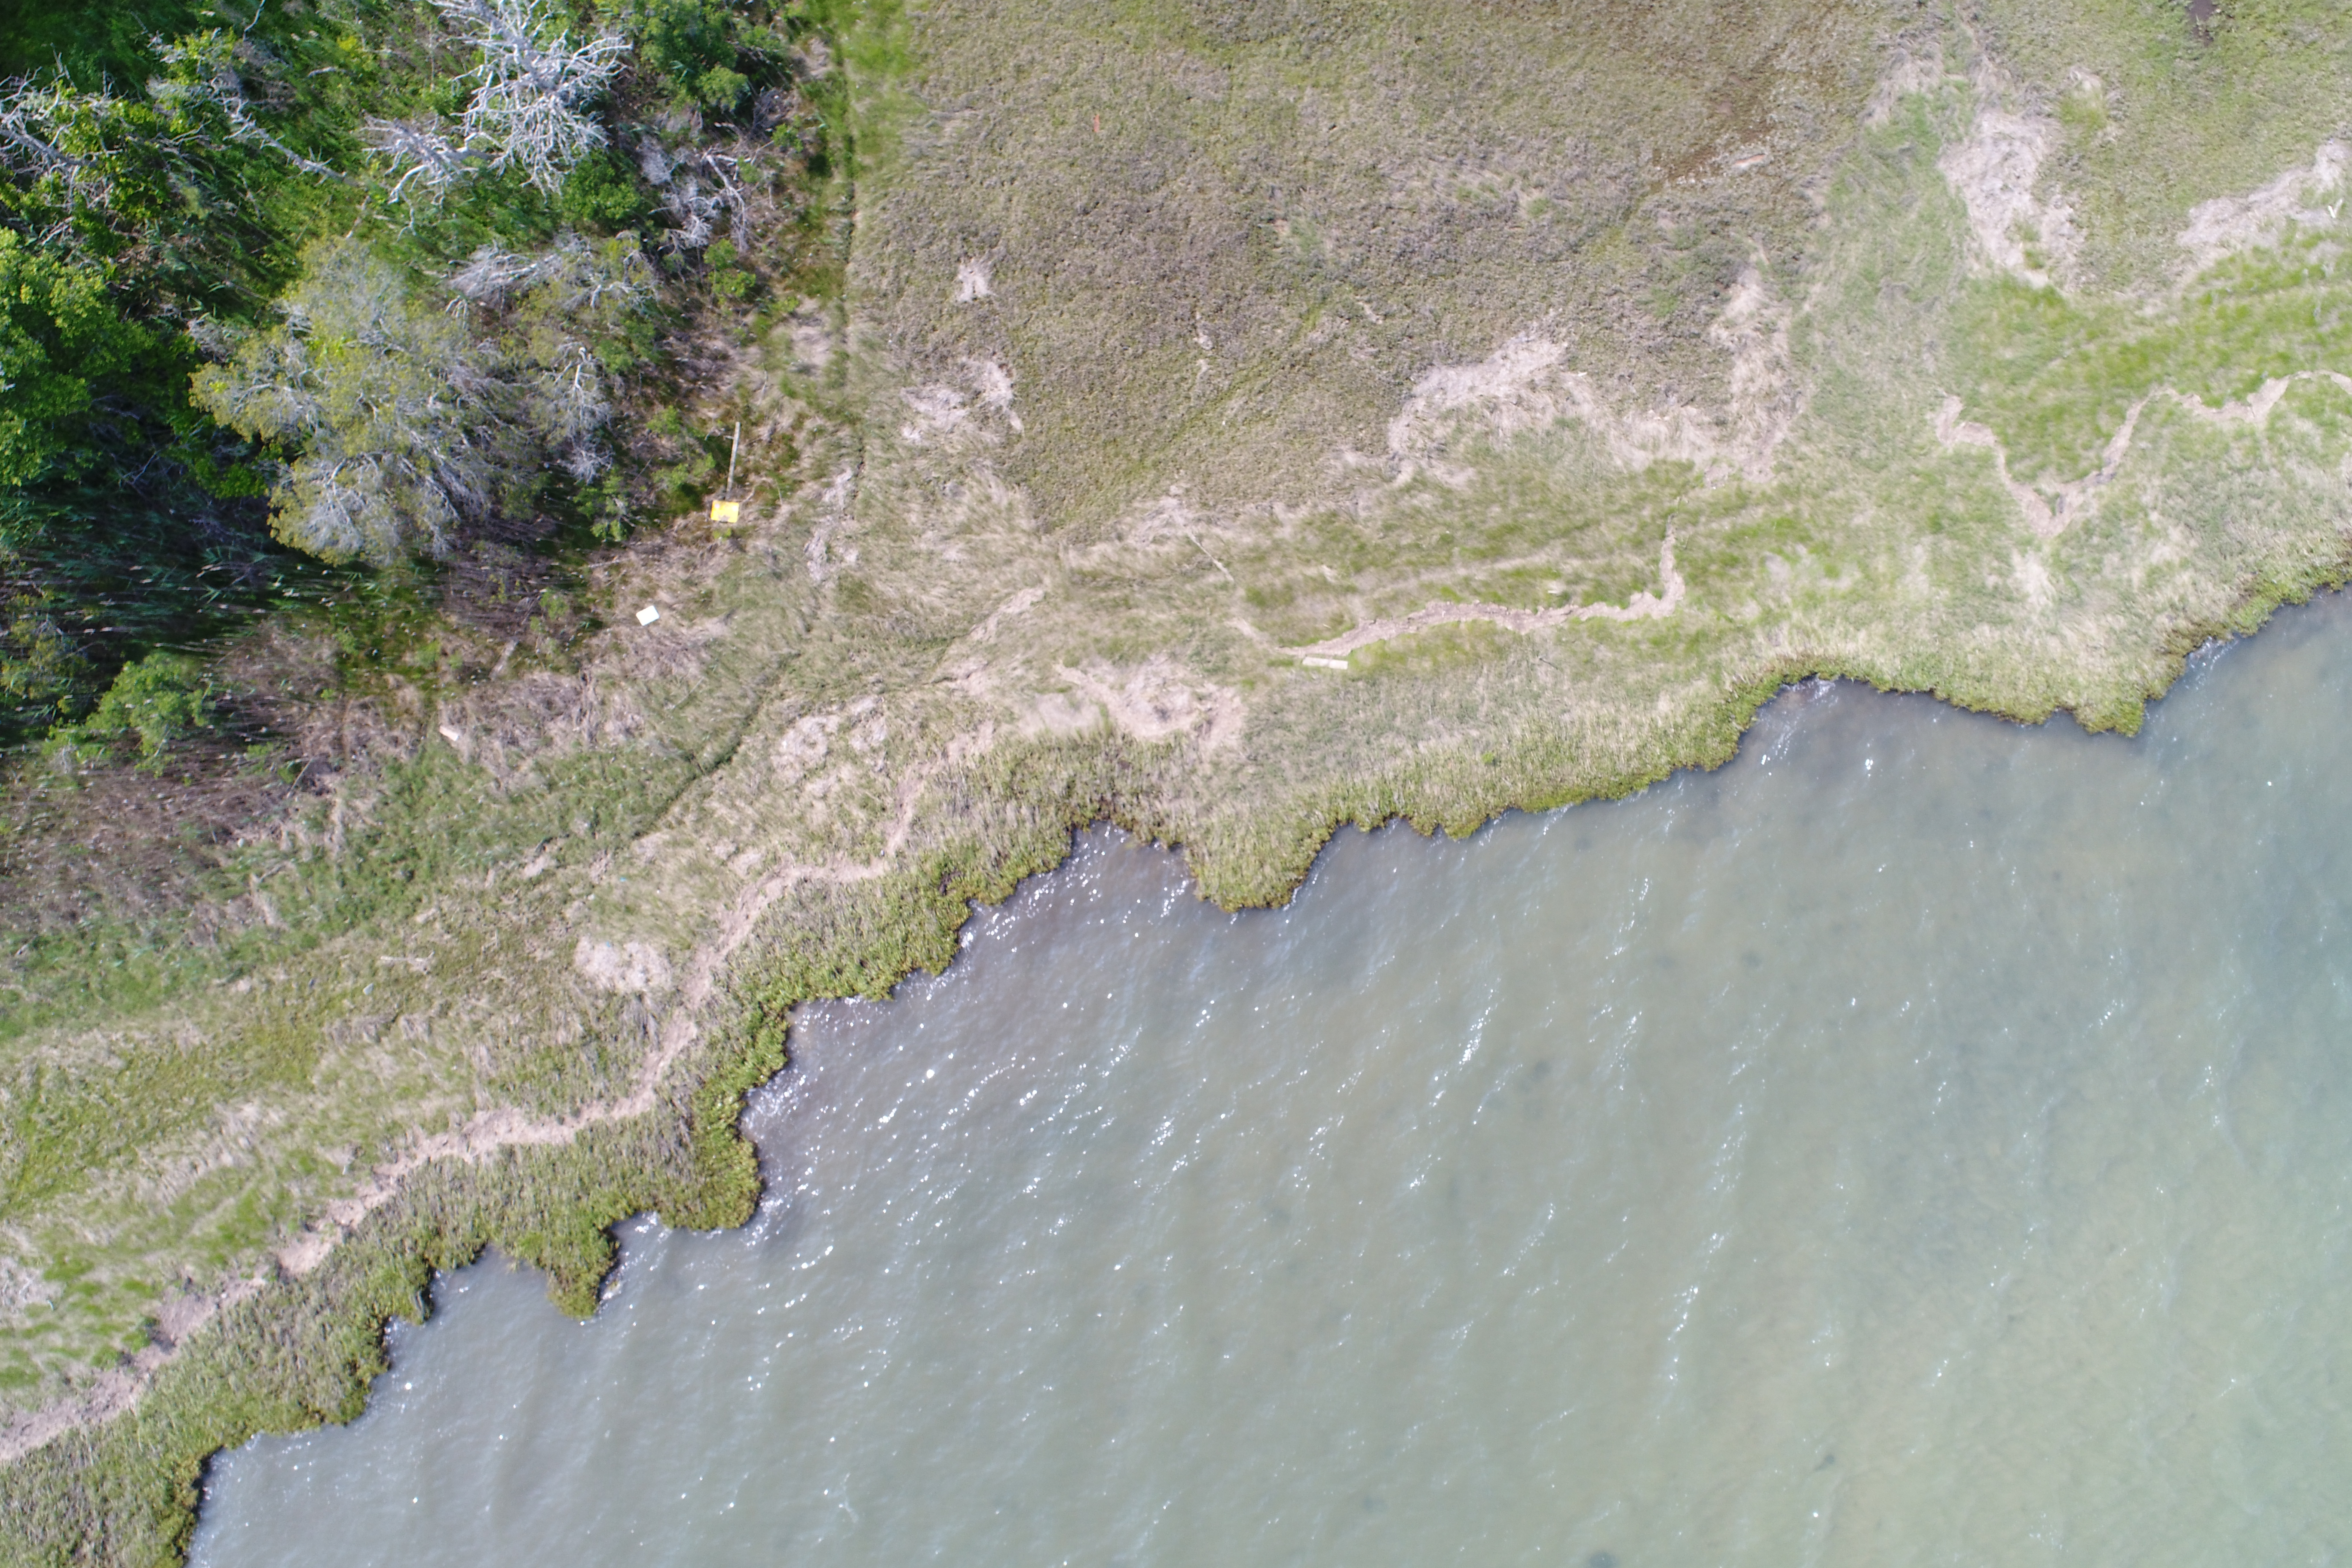
\includegraphics[width=\textwidth]{images/site_assateague_island_aerial.JPG} \\
        (b)
    \end{minipage}
    
    \vspace{1.5em} % Spazio verticale tra le righe

    % --- Seconda riga: (c) e (d) ---
    % Manteniamo [b] per coerenza. Uniformiamo la dimensione della mappa (d).
    \begin{minipage}[b]{0.45\textwidth}
        \centering
        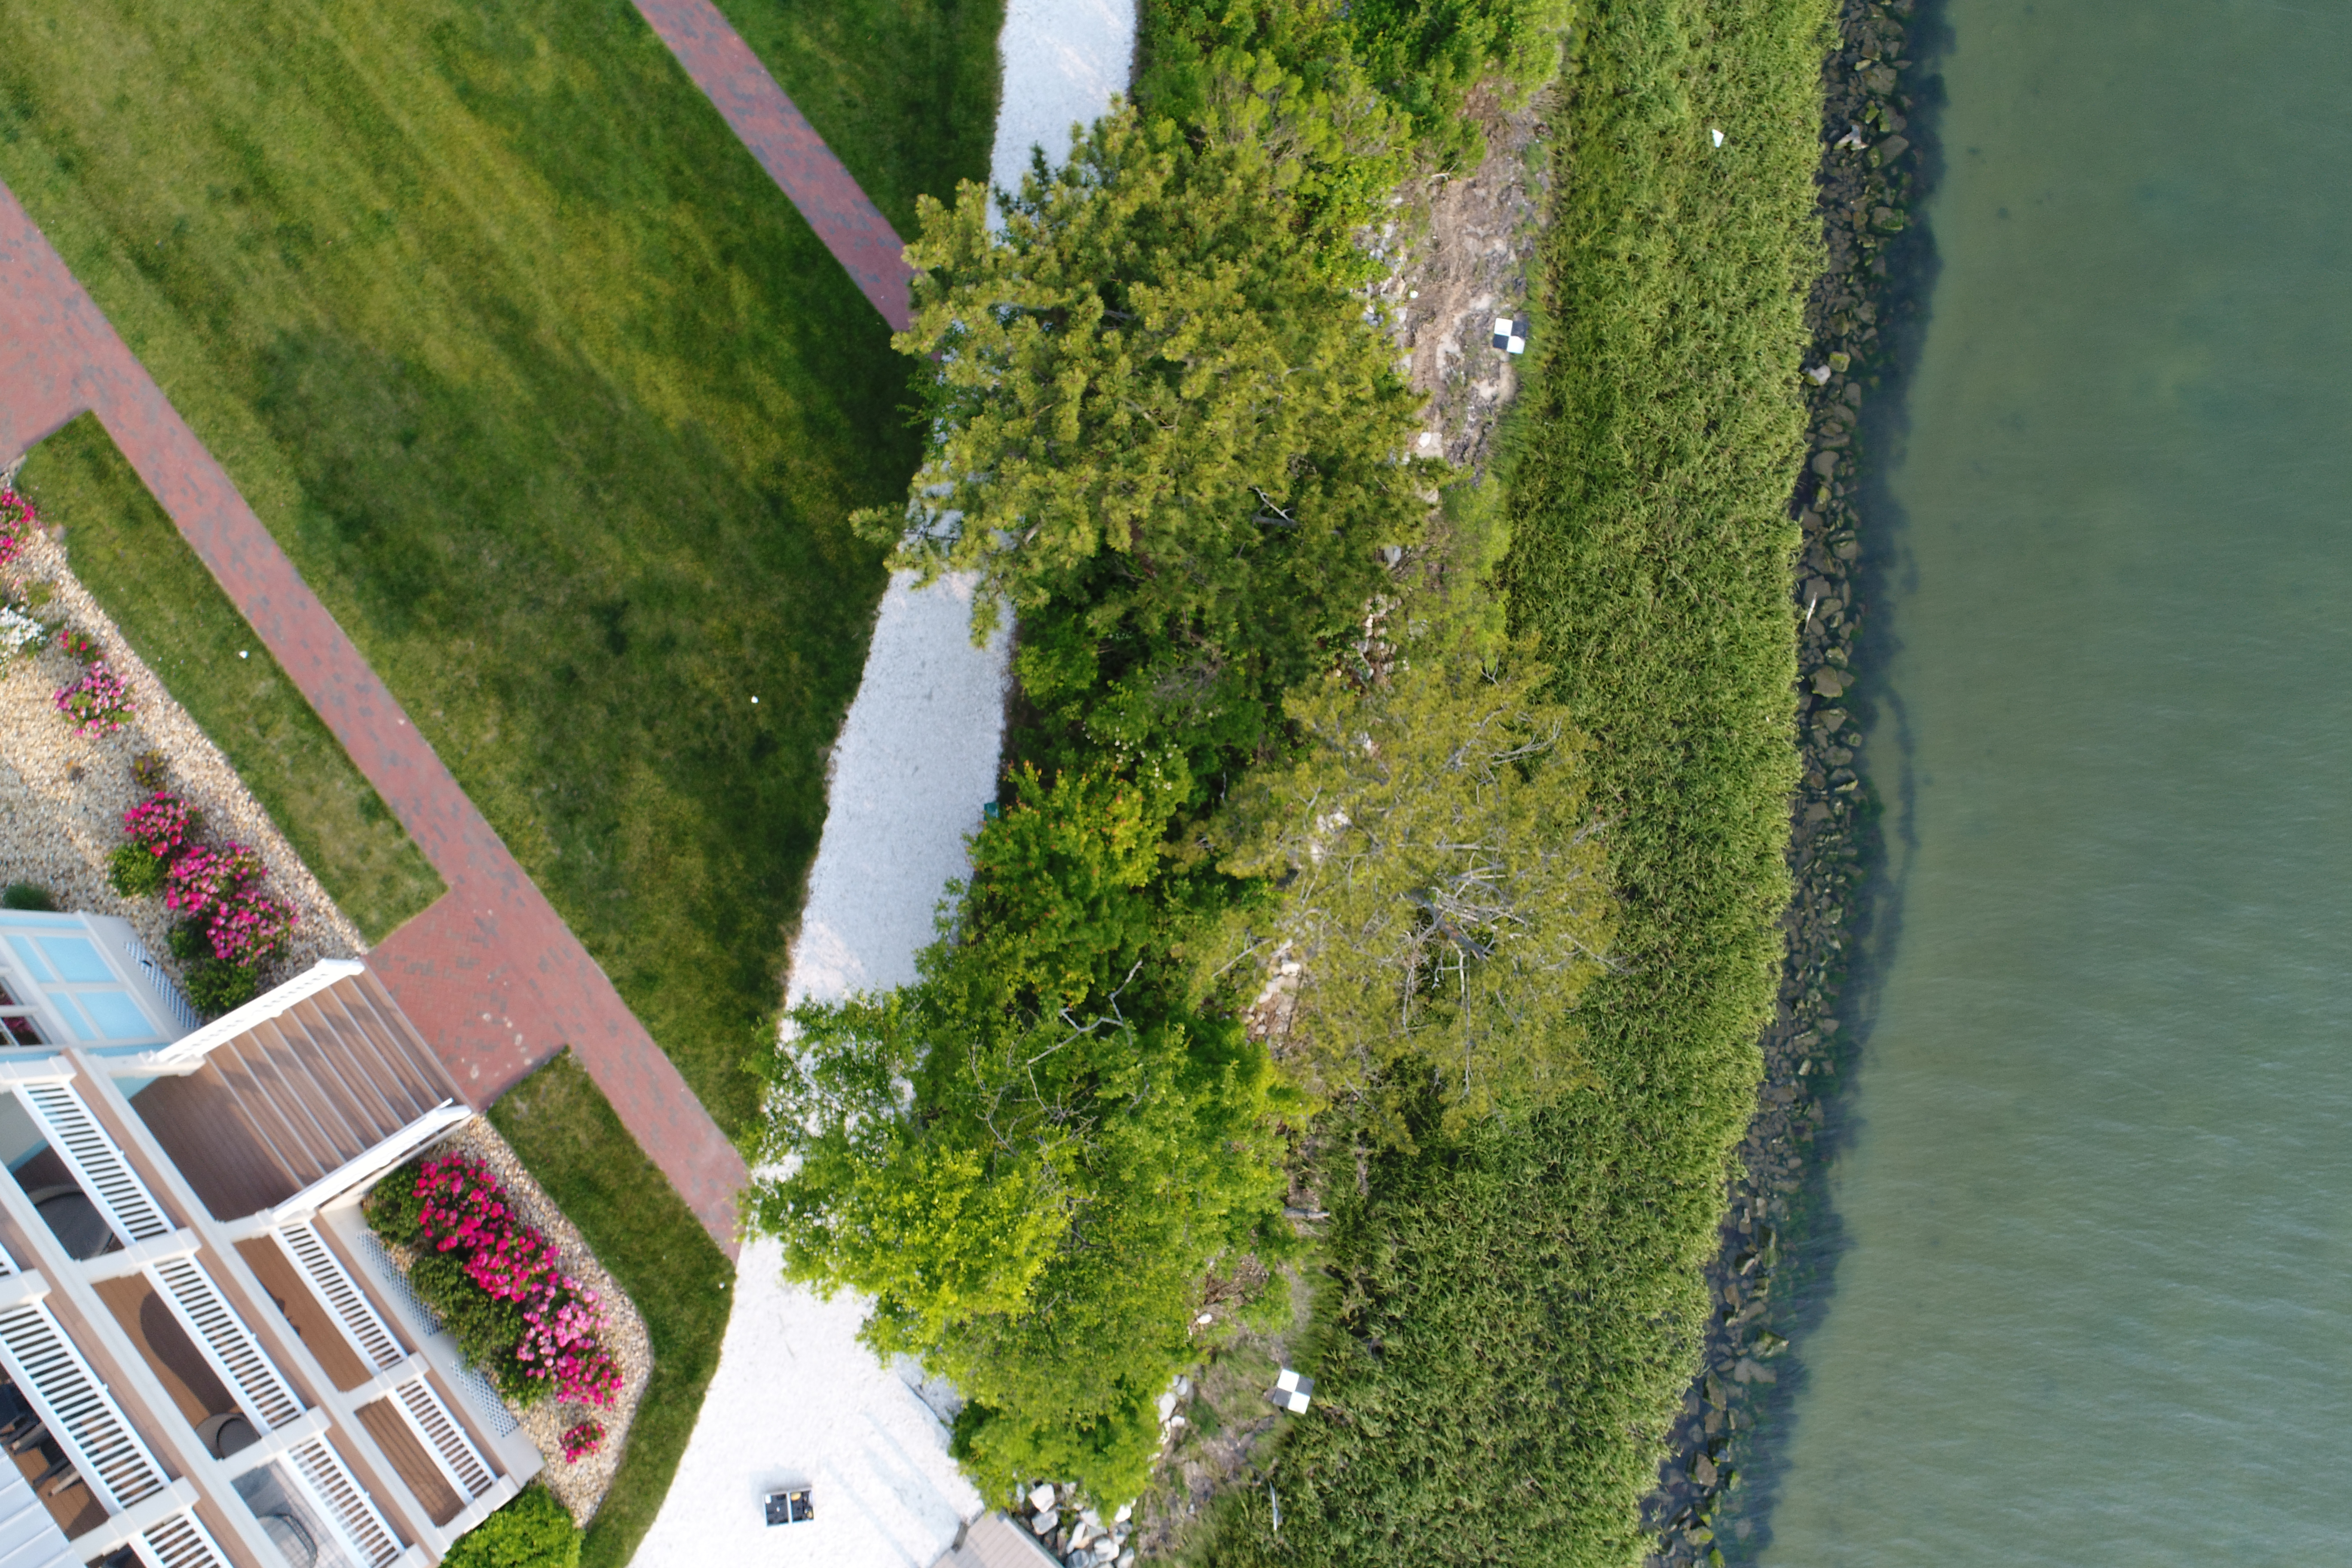
\includegraphics[width=\textwidth]{images/site_sunset_island_aerial.JPG} \\
        (c)
    \end{minipage}
    \hfill
    \begin{minipage}[b]{0.20\textwidth}
        \centering
        % La mappa (d) ora ha la stessa larghezza delle altre immagini per simmetria
        \includegraphics[width=\textwidth]{images/study_area_chesapeake_bay_map.png} \\
        (d)
    \end{minipage}

    \caption{Representative aerial images of the study sites: (a) Poplar Island, (b) Assateague Island, (c) Sunset Island, and (d) geographic context within the Chesapeake Bay region. Note: Map lines delineate study areas and do not necessarily depict accepted national boundaries.}
    \label{fig:siti}
\end{figure}

\subsection{UAV Image Acquisition}

High-resolution imagery was acquired via UAV surveys at Poplar, Assateague, and Sunset Islands (Maryland, USA) in December 2024. Four flight missions per site covered approximately 400 m × 400 m using a DJI Phantom 3 Professional (DJI-P3P) equipped with an integrated DJI FC300X RGB camera and an additional multispectral sensor. Flight plans, managed via Pix4D Capture, maintained 80\% longitudinal and 60\% lateral overlap at a constant 40-meter altitude to ensure consistent spatial coverage. Reduced flight autonomy due to the payload was accounted for during planning. The RGB and multispectral imagery achieved Ground Sample Distances (GSD) of approximately 1.8 cm and 2.8 cm, respectively, supporting fine-scale environmental analyses.

The acquired imagery, encompassing marshland, watercourses, and vegetated areas, formed the basis of a texture-based dataset. A Python workflow was used to manually extract and label 128×128 pixel patches of key environmental classes from the orthomosaics. For each class, 40 patches per site were selected to create a `clean' dataset of high-quality samples, stored in 8-bit per channel RGB PNG format.

\subsection{Classification Dataset and Data Organization}

The dataset is organized by geographic area using specific land cover classes: \textit{low\_veg} (herbaceous vegetation), \textit{trees} (woody vegetation), \textit{water} (tidal channels and wetlands, present in Poplar and Assateague), and \textit{garden} (anthropogenic green areas, present only in Sunset). This organization reflects site-specific ecology: Poplar and Assateague feature natural aquatic environments, while Sunset represents a residential area with anthropogenic elements.
The naming convention follows the pattern: \texttt{\{noise\_type\}\_\{intensity\}\_\{dimension\}\_\{location\}}. Rationale and noise descriptions are provided in the Supplementary Materials.

To investigate dataset size effects, three variants were created: \textit{Mini} ($\sim$5 images per class, testing extreme scarcity); \textit{Small} ($\sim$10 images per class, moderate limitation); and \textit{Original} ($\sim$40 images per class, full dataset). An \textit{Augmented} variant ($\sim$100 images per class) utilizing geometric transformations was also tested. However, as preliminary results showed negligible accuracy gains ($<1\%$) over the \textit{Original} set, indicating a learning plateau, this variant was excluded to optimize efficiency without compromising validity.

Feature extraction robustness was evaluated by corrupting the clean dataset with five noise types at varying intensities (low, moderate, high), simulating common UAV signal degradations. This process resulted in the variants summarized in Table~\ref{tab:noise_summary}.

\begin{table}[t]
    \centering
    \caption{Noise Dataset Summary}
    \label{tab:noise_summary}
    \begin{tabular}{l c c c c}
        \toprule
        \textbf{Noise Type} & \textbf{Low Level} & \textbf{Moderate Level} & \textbf{High Level} & \textbf{Total Variants} \\
        \midrule
        \textbf{Gaussian} & - & $\sigma=30$ & $\sigma=50$ & 2 \\
        \textbf{Poisson} & - & $\lambda=60$ & $\lambda=100$ & 2 \\
        \textbf{Salt \& Pepper} & 5\% & 15\% & 25\% & 3 \\
        \textbf{Speckle} & $\sigma^2=15$ & $\sigma^2=35$ & $\sigma^2=55$ & 3 \\
        \textbf{Uniform} & $r=10$ & $r=25$ & $r=40$ & 3 \\
        \textbf{Clean} & -- & -- & -- & 1 \\
        \midrule
        \textbf{TOTAL} & & & & \textbf{14 datasets} \\
        \bottomrule
    \end{tabular}
\end{table}

\subsection{Feature Extraction and Feature Selection}
Feature extraction is critical for transforming raw RGB data into numerical representations for machine learning. Three methodological approaches were compared. The first, serving as a standard baseline, extracts 18 statistical descriptors per channel (54 total), including first-order statistics, shape indicators, robust quantile measures, and texture features (detailed in Table~\ref{tab:stat_features}).

\subsubsection{Wavelet Scattering Transform (WST)}
The second approach, the Wavelet Scattering Transform (WST) \cite{Bruna2013Invariant}, provides a multi-scale, translation-invariant representation via cascaded wavelet modulus operators. Unlike CNNs, WST uses predefined Morlet wavelets without filter learning. Implemented via Kymatio \cite{andreux2020kymatio}, the recursive scattering operator $S$ is defined as:

\begin{align}
    \textbf{Order 0:} & \quad S_0 x = x \star \varphi_J \\
    \textbf{Order 1:} & \quad S_1 x(\lambda_1) = |x \star \psi_{\lambda_1}| \star \varphi_J \\
    \textbf{Order 2:} & \quad S_2 x(\lambda_1, \lambda_2) = ||x \star \psi_{\lambda_1}| \star \psi_{\lambda_2}| \star \varphi_J
\end{align}

where $\varphi_J$ is a low-pass filter (father wavelet), $\psi_{\lambda}$ are Morlet wavelets parameterized by scale $j$ and orientation $\theta$, $\star$ denotes convolution, and $|\cdot|$ is the complex modulus.
WST generates $\sim$81 coefficients per channel. Computing mean and standard deviation yields $\sim$162 features per channel ($\sim$486 total), capturing multi-scale spatial information and directional orientations. Key advantages include invariance to small deformations, coefficient stability, geometric interpretability, and the absence of parameter training.

The third, hybrid approach combines the 54 statistical features with WST features, leveraging complementary pointwise intensity properties and multi-scale spatial patterns. Regardless of the method, all features were normalized using scikit-learn's \texttt{StandardScaler} \cite{scikit-learn}:
\[
z = (x - \mu) / \sigma
\]
where $\mu$ and $\sigma$ are computed on the training set to prevent data leakage.

\begin{table}[t]
    \centering
    \caption{Complete set of statistical features (18 per RGB channel, 54 total).}
    \label{tab:stat_features}
    \begin{tabular}{p{3cm} p{4cm} p{8cm}}
        \toprule
        \textbf{Category} & \textbf{Feature} & \textbf{Description} \\
        \midrule
        Basic Statistics & Mean ($\mu$) & Central value of the intensity distribution \\
         & Standard Deviation ($\sigma$) & Dispersion of intensity values \\
         & Variance ($\sigma^2$) & Square of the standard deviation \\
         & Minimum & Lowest pixel intensity in the channel \\
         & Maximum & Highest pixel intensity in the channel \\
         & Range & Difference between maximum and minimum values \\
        \midrule
        Shape Statistics & Skewness & Asymmetry of the distribution relative to the mean \\
         & Kurtosis & Tail weight relative to a normal distribution \\
         & Coefficient of Variation (CV) & Normalized dispersion: $\sigma / \mu$ \\
        \midrule
        Robust/Percentile Stats & 10th Percentile & Lower quantile of the intensity distribution \\
          & 25th Percentile & First quartile of the intensity distribution \\
          & Median (50th) & Central value less sensitive to outliers \\
          & 75th Percentile & Third quartile of the intensity distribution \\
          & 90th Percentile & Upper-tail quantile \\
          & Interquartile Range (IQR) & Difference between 75th and 25th percentile \\
          & Median Absolute Deviation (MAD) & Median of absolute deviations from the median \\
        \midrule
        Spatial Features & Gradient Mean & Mean spatial gradient (Sobel-based) \\
         & Edge Density & Percentage of edge pixels (Laplacian thresholding) \\
        \bottomrule
    \end{tabular}
\end{table}

\subsubsection{Features Selection} 
Given the high dimensionality of the feature space, a feature selection phase was applied to identify the most informative subset and reduce the risk of overfitting. The SelectKBest algorithm from scikit-learn was used, with scoring based on Mutual Information (MI). Mutual information measures the non-linear dependency between each feature $X_i$ and the target variable $Y$:
\[
\text{MI}(X_i; Y) = \sum_{x_i} \sum_{y} p(x_i, y) \log\left(\frac{p(x_i, y)}{p(x_i)p(y)}\right)
\]
where $p(x_i, y)$ is the joint distribution and $p(x_i)$ and $p(y)$ are the marginal distributions
Mutual information offers significant advantages over linear methods such as Pearson correlation, as it captures non-linear dependencies, does not assume a Gaussian distribution, is invariant under monotonic transformations, and has a range of $[0, \infty]$, with $0$ indicating independence \cite{scikit-learn}.
Four values,  2, 5, 10, 20 of $k$ were systematically tested. Experimental analysis revealed that \textbf{$k=5$} provides the best compromise between accuracy (0.930) and model complexity. Feature selection is always performed on the training set and applied to the test set to avoid selection bias.

\subsection{Classification through Random Forest}

Random Forest \cite{Breiman2001} is an ensemble method that constructs multiple decision trees via bagging and random feature selection ($\sqrt{p}$), with final predictions determined by majority voting. It was selected for its reduced variance, robustness to overfitting, handling of non-linear interactions, and interpretability.
The model employed an adaptive configuration (Table~\ref{tab:rf_hyperparams}), where \texttt{n\_estimators} was scaled proportionally to dataset size. This approach balances generalization with computational cost, preventing overfitting in smaller datasets while maximizing prediction stability in larger ones.

\begin{table}[t]
    \centering
    \caption{Random Forest hyperparameters and configuration details.}
    \label{tab:rf_hyperparams}
    \begin{tabular}{p{4cm} p{9cm}}
    \toprule
    \textbf{Hyperparameter} & \textbf{Value / Description} \\
    \midrule
    \textbf{n\_estimators} & Mini: 3 trees; Small: 10 trees; Original: 50 trees \\
    \textbf{criterion} & Gini impurity \\
    \textbf{max\_depth} & None (trees grown until pure leaves) \\
    \textbf{min\_samples\_split} & 2 \\
    \textbf{min\_samples\_leaf} & 1 \\
    \textbf{max\_features} & \texttt{sqrt} ($\sqrt{p}$ features considered at each split) \\
    \textbf{bootstrap} & True \\
    \textbf{random\_state} & 42 (for reproducibility) \\
    \bottomrule
    \end{tabular}
\end{table}

\subsubsection{Model Validation}
Validation employed 5-fold Stratified Cross-Validation (SCV) across all 1,512 models to ensure stable performance estimates and mitigate partition variability \cite{witten2016valutazione, kohavi1995crossvalidation, szeghalmy2023scv}.  SCV preserves class distributions within each disjoint fold (80\% training, 20\% validation), which is critical for low-data regimes. We recorded \texttt{cv\_mean\_accuracy} and \texttt{cv\_std} to assess model stability, where lower deviation indicates consistency across splits. Finally, a separate 80/20 stratified Train/Test partition was established for conclusive evaluation.

\subsubsection{Evaluation Metrics}
Performance was assessed using the following metrics, chosen to capture overall correctness, specificity, sensitivity, and stability \cite{witten2016valutazione,Powers2011}:

\textbf{Accuracy}:
\[
\text{Acc} = \frac{\text{TP} + \text{TN}}{\text{TP} + \text{TN} + \text{FP} + \text{FN}}
\]
Ratio of correct predictions, appropriate for the balanced class distribution.

\textbf{Precision (per class)}:
\[
\text{Prec} = \frac{\text{TP}}{\text{TP} + \text{FP}}
\]
Measures classifier specificity.

\textbf{Recall (per class)}:
\[
\text{Rec} = \frac{\text{TP}}{\text{TP} + \text{FN}}
\]
Measures classifier sensitivity.

\textbf{F1-Score (per class)}:
\[
\text{F1} = 2 \cdot \frac{\text{Prec} \cdot \text{Rec}}{\text{Prec} + \text{Rec}}
\]
Harmonic mean providing a balanced single metric.

\textbf{Confusion Matrix}:\\
Matrix $C$ where $C_{ij}$ denotes samples of class $i$ predicted as $j$, detailing misclassifications.

\textbf{Cross-Validation Metrics}:\\
Mean accuracy and standard deviation across folds to indicate stability.

\subsection{Statistical Analysis}
The statistical analysis aims to:
\begin{enumerate}
    \item \textbf{Quantify comparative robustness} across 6 noise types (Gaussian, Poisson, Salt\&Pepper, Speckle, Uniform) at increasing intensities;
    \item \textbf{Evaluate data efficiency} in scenarios of scarcity (mini: $\sim5$ img/class), moderate (small: $\sim15$), and standard availability (original: $\sim40$);
    \item \textbf{Determine specific configurations} where WST or Hybrid methods yield statistically significant advantages;
    \item \textbf{Separate statistical significance from practical relevance} through effect size analysis.
\end{enumerate}
Non-parametric tests with multiple comparison corrections were applied to rigorously evaluate the methods, controlling for spatial autocorrelation through geographic aggregation.

\subsubsection{Dataset Construction and Full Factorial Experimental Design}
The study employs a fully crossed factorial design yielding $1,512$ experiments. Each experiment is defined by six independent factors: geographic area, dataset size, feature extraction method, K-best dimensionality, noise type, and intensity.
The base grid consists of 108 configurations ($3 \text{ areas} \times 3 \text{ sizes} \times 3 \text{ methods} \times 4 \text{ K-values}$), which were expanded according to the noise families and intensity levels summarized in Table~\ref{tab:dataset_factors_unified} and Table~\ref{tab:noise_intensities}. This resulted in specific subsets for Clean (108), Gaussian (216), Poisson (216), Salt \& Pepper (324), Speckle (324), and Uniform (324) conditions.

Reproducibility was ensured by explicitly controlling all randomness sources. Fixed seeds (\texttt{Python}=42, \texttt{NumPy}=42, \texttt{random\_state}=42) were used for all generators, and processing steps were strictly ordered.
To reduce spatial autocorrelation, results were aggregated by averaging metrics across the three geographic locations, condensing the $1,512$ raw experiments into $504$ configuration-level observations. Table~\ref{tab:evaluation_metrics} lists the metrics extracted for analysis.

\begin{table}[t]
    \centering
    \caption{Summary of the factors defining the full experimental dataset.}
    \label{tab:dataset_factors_unified}
    \begin{tabular}{llc}
        \toprule
        \textbf{Factor} & \textbf{Values} & \textbf{Levels} \\
        \midrule
        Geographic Areas & Assateague, Poplar, Sunset & 3 \\
        Dataset Sizes & mini ($\sim$5 img/class), small ($\sim$15), original ($\sim$40) & 3 \\
        Feature Methods & advanced\_stats, wst, hybrid & 3 \\
        K-best Values & 2, 5, 10, 20 & 4 \\
        Noise Types & clean, gaussian, poisson, saltpepper, speckle, uniform & 6 \\
        Noise Intensities & See Table~\ref{tab:noise_intensities} & -- \\
        Land Cover Classes & 3 per area (Sunset: garden replaces water) & -- \\
        \bottomrule
    \end{tabular}
\end{table}

\begin{table}[t]
    \centering
    \caption{Noise families and intensity levels used to generate corrupted dataset variants.}
    \label{tab:noise_intensities}
    \begin{tabular}{lcl}
        \toprule
        \textbf{Noise Type} & \textbf{Intensity Levels} & \textbf{Parameters} \\
        \midrule
        Clean & 1 & No corruption \\
        Gaussian & 2 & $\sigma = 30, 50$ \\
        Poisson & 2 & $\lambda = 40, 60$ \\
        Salt \& Pepper & 3 & $p = 5\%, 15\%, 25\%$ \\
        Speckle & 3 & $\sigma^2 = 15, 35, 55$ \\
        Uniform & 3 & $r = 10, 25, 40$ \\
        \bottomrule
    \end{tabular}
\end{table}

\begin{table}[t]
    \centering
    \caption{Performance metrics extracted for each of the 1,512 experiments.}
    \label{tab:evaluation_metrics}
    \begin{tabular}{lp{9cm}}
        \toprule
        \textbf{Metric} & \textbf{Description} \\
        \midrule
        Test Accuracy & Computed on the 20\% hold-out test set \\
        Macro-averaged F1-score & Weighted harmonic mean of Precision and Recall over the 3 classes \\
        Macro-averaged Precision & Average class-wise Precision, unweighted by class frequency \\
        Macro-averaged Recall & Average class-wise Recall, unweighted by class frequency \\
        Cross-validation Scores & 5-fold stratified CV accuracy values (mean and standard deviation) \\
        Confusion Matrix & $3 \times 3$ matrix showing class-wise prediction distribution \\
        \bottomrule
    \end{tabular}
\end{table}

\subsection{Structure of the Analytical Framework} 

\subsubsection{Pairwise Comparisons Between Methods}

To rigorously quantify relative performance, pairwise deltas on the Macro-F1 metric were calculated for each configuration $i \in \{1, \ldots, 168\}$ relative to the Advanced Stats baseline:

\[
\begin{aligned}
    \Delta_{\text{WST},i} &= \text{Macro-F1}_{\text{WST}}(i) - \text{Macro-F1}_{\text{AdvStats}}(i) \\
    \Delta_{\text{Hybrid},i} &= \text{Macro-F1}_{\text{Hybrid}}(i) - \text{Macro-F1}_{\text{AdvStats}}(i)
\end{aligned}
\]

In total, 336 comparisons were performed. 
A positive delta ($\Delta > 0$) indicates improvement over the baseline. Aggregated statistics ($\mathbb{E}[\Delta]$, $\text{Std}[\Delta]$, $\text{Median}[\Delta]$) were computed to assess average performance and stability. To determine statistical significance, the following 4-step workflow was applied. 

\paragraph{Step 1: Normality Assessment via Shapiro–Wilk Test}
The Shapiro–Wilk test \cite{Shapiro1965Analysis} was applied to the 168 deltas for each comparison to assess Gaussianity ($H_0: \text{deltas} \sim \mathcal{N}$). The test statistic is defined as:

\[W = \frac{\left(\sum_{i=1}^{n} a_i x_{(i)}\right)^2}{\sum_{i=1}^{n} (x_i - \bar{x})^2}\]

As summarized in Table~\ref{tab:shapiro_results}, normality was rejected for both comparisons ($p < 0.05$), necessitating non-parametric statistical methods.

\begin{table}[t]
    \centering
    \caption{Shapiro–Wilk normality test results for pairwise deltas.}
    \label{tab:shapiro_results}
    \begin{tabular}{lccc}
        \toprule
        \textbf{Comparison} & \textbf{Sample Size} & \textbf{$p$-value} & \textbf{Normality Decision} \\
        \midrule
        WST vs AdvStats     & 168                  & 0.0213             & Not normal ($p < 0.05$) \\
        Hybrid vs AdvStats  & 168                  & 0.0087             & Not normal ($p < 0.05$) \\
        \bottomrule
    \end{tabular}
\end{table}

\paragraph{Step 2: Selection and Execution of the Wilcoxon Signed-Rank Test}
Given the non-normal distributions, the Wilcoxon signed-rank test \cite{Wilcoxon1945Individual} was selected to assess if the median difference differs significantly from zero ($H_0: \text{median}=0$). The test statistic $W = \min(R^+, R^-)$ is based on the rank sums of positive and negative deltas. This method is robust to outliers and leverages the paired nature of the data to reduce the influence of confounding factors.

\paragraph{Step 3: Multiple Comparison Correction (FDR)}
To control for Type I error inflation across $k=4$ tests (2 methods $\times$ 2 metrics), the False Discovery Rate (FDR) was adjusted using the Benjamini–Hochberg procedure \cite{Benjamini1995}. Critical values are adjusted as:

\[
p_{\text{FDR}}(i) = \min\left(1, \, p_{(i)} \times \frac{k}{i}\right)
\]

Joint correction was applied to ensure that the expected proportion of false discoveries does not exceed $\alpha=0.05$, balancing statistical power with inferential robustness.

\paragraph{Step 4: Effect Size Estimation and Statistical Power Assessment}
To quantify practical magnitude independent of sample size, Cohen's $d$ \cite{Cohen1988} was computed using Hedge's $g$ correction for bias reduction:

\[
d = \frac{\mu(\Delta)}{\sigma(\Delta)}, \quad g = d \times \left(1 - \frac{3}{4n - 9}\right)
\]

Effect sizes are categorized as small ($|d| < 0.2$), medium ($0.5 \leq |d| < 0.8$), or large ($|d| \geq 0.8$). Bootstrap 95\% confidence intervals (1,000 iterations) were generated to estimate uncertainty:

\[
\text{CI}_{95\%}(d) = \left[ \text{percentile}_{2.5}(d_b), \, \text{percentile}_{97.5}(d_b) \right]
\]

With $n=168$, the study has adequate power to detect medium effects. Observed results showed a negligible effect for WST ($d=-0.075$, $p=0.083$) and a small but significant effect for Hybrid ($d=0.156$, $p=0.039$). 

\subsubsection{Noise Robustness Analysis}

Robustness to noise was evaluated by modeling performance degradation as a function of noise intensity using a linear regression framework. For each combination of \texttt{noise\_type}, dataset size, $k$ value, and feature extraction method, the following model was fitted:

\[
\text{Accuracy} = \beta_0 + \beta_1 \times \text{Intensity} + \epsilon
\]

Here, $\beta_0$ represents the theoretical accuracy at zero noise, while $\beta_1$ (slope) quantifies the degradation rate. Ordinary least squares regression was performed using \texttt{scipy.stats.linregress} \cite{Virtanen2020SciPy} to extract $\beta_1$ as the primary robustness indicator, alongside $R^2$ and $p$-values for validation.
The interpretation is straightforward: slopes near zero indicate stability, while negative slopes reflect degradation. Consequently, methods with less negative slopes are considered more robust.

To quantify relative robustness, the percentage difference in slope magnitude was computed as:
\[
\text{Relative Robustness} = \frac{|\beta_1^{\text{Advanced}}| - |\beta_1^{\text{Hybrid}}|}{|\beta_1^{\text{Advanced}}|} \times 100\%
\]
For instance, a reduction in slope magnitude from $0.002068$ to $0.000894$ corresponds to a $\approx 56.8\%$ improvement in stability. This metric standardizes the comparison across approaches. All $\sim150$ regression results, including slope, intercept, $R^2$, and standard error, were archived in \texttt{noise\_robustness\_slopes.csv} for analysis.

\subsubsection{Data Scarcity Analysis}
Performance under limited data was assessed via a retention metric, defined for each method and dataset size as:

\[
\text{Retention}(\text{size}) = \left[\frac{\text{Accuracy}(\text{size})}{\text{Accuracy}(\text{original})}\right] \times 100
\]

The \textit{Original} dataset ($\sim$40 images/class) serves as the 100\% baseline. Retention quantifies performance preservation in two reduced regimes: \textit{Mini} ($\sim$5 images/class) and \textit{Small} ($\sim$15 images/class).
Scores were averaged across noise types and $k$ values, with computed standard deviations. Methods maintaining retention $>90\%$ were deemed data-efficient, while those below $80\%$ indicated strong dependence on larger training sets. High retention in the \textit{Mini} setting implies robust generalization from few examples, whereas low retention signals sensitivity to scarcity, likely due to overfitting or high-dimensional feature reliance.
Results ($\sim$450 observations) were consolidated into a CSV file, detailing specific retention percentages per configuration alongside aggregated statistics.

\subsubsection{Global Performance Distribution Analysis} 

To characterize global performance trends, we examined the aggregated distribution of classification metrics across the complete factorial design. For each configuration, Accuracy and Macro-F1 computed on held-out test partitions were summarized using descriptive statistics. This representation facilitates a distribution-level comparison, highlighting central tendency, dispersion, and unstable cases. Unlike targeted comparisons (e.g., pairwise deltas or robustness slopes), this analysis provides an integrated view of global variability across heterogeneous conditions. It effectively identifies systematic shifts in median performance, method overlap, and sensitivity to challenging scenarios like high-intensity noise or data scarcity, offering a holistic assessment of generalization across the experimental landscape.

\subsubsection{Feature Selection and K-Best Dimensionality Analysis}

To assess performance as a function of dimensionality, we conducted a controlled analysis using \texttt{SelectKBest} based on mutual information scores. Four feature budgets were evaluated ($K = 2, 5, 10, 20$), ranging from extremely compact to moderately enriched representations.For each $K$, performance was averaged across all noise and dataset conditions to estimate how discriminative information accumulates. This isolates dimensionality effects, identifying diminishing returns, redundancy, or method-specific sensitivity to pruning. Unlike noise or scarcity experiments which probe external robustness, this analysis focuses on intrinsic efficiency, revealing the minimum features required for stability and the rate of improvement. This framework enables a principled comparison of the compactness and discriminative density of the three feature spaces.The complete experimental design ensures a systematic and reproducible evaluation across diverse regimes. The integration of statistical hypothesis testing, effect size quantification, and robustness analysis guarantees that the findings reported in the following sections are statistically rigorous and practically interpretable.

\section{Results}

A total of 1,512 experiments were conducted and aggregated into 504 configurations to enable robust comparison between the three feature extraction strategies. 

\subsection{Pairwise performance differences ($\Delta(Macro-F1)$)}

Pairwise Macro-F1 deltas were computed for WST vs. Advanced Statistics and Hybrid vs. Advanced Statistics across 168 experimental conditions. The analysis evaluated distributional properties, normality (Shapiro–Wilk), statistical significance (FDR-corrected Wilcoxon signed-rank test), and effect sizes (Cohen’s $d$). Table~\ref{tab:unified_stats} summarizes the statistical outcomes, while Figure~\ref{fig:delta_heatmap} provides a visual heatmap of the deltas.

\begin{table*}[t]
    \centering
    \caption{Statistical comparison between WST/Hybrid and Advanced Statistics.}
    \label{tab:unified_stats}
    \small
    \begin{tabular}{@{}llcccccc@{}}
        \toprule
        \textbf{Metric} & \textbf{Comparison} & \textbf{Mean $\Delta$} & \textbf{Median $\Delta$} & 
        \textbf{Shapiro-Wilk $p$} & \textbf{Cohen's $d$} & \textbf{$p$ (FDR)} & \textbf{Sig.} \\
        \midrule
        \multicolumn{8}{l}{\textit{Macro-F1 Score}} \\
        \midrule
        & WST vs AdvStats    
            & $-0.0106 \pm 0.1410$ 
            & $-0.0005$ 
            & 0.0213 (non-normal)
            & $-0.075$ 
            & 0.0825 
            & ns \\
        & Hybrid vs AdvStats 
            & $+0.0171 \pm 0.1092$ 
            & $0.0000$ 
            & 0.0087 (non-normal)
            & $+0.156$ 
            & \textbf{0.0390} 
            & * \\
        \midrule
        \multicolumn{8}{l}{\textit{Accuracy}} \\
        \midrule
        & WST vs AdvStats    
            & $-0.0103$ 
            & --- 
            & --- 
            & $-0.089$ 
            & 0.0898 
            & ns \\
        & Hybrid vs AdvStats 
            & $+0.0144$ 
            & --- 
            & --- 
            & $+0.159$ 
            & 0.0518 
            & ns \\
        \bottomrule
    \end{tabular}
\end{table*}

\subsubsection{WST vs Advanced Statistics}

The WST–Advanced comparison reveals a slightly negative mean delta ($-0.0106$) and a median near zero. Normality was rejected ($p=0.0213$), and the FDR-corrected Wilcoxon test yielded a non-significant p-value of 0.0825. The negligible effect size ($d=-0.075$) confirms the lack of substantial difference. Visually, the heatmap displays predominately yellow-to-light-orange tones, with red cells appearing under clean or low-noise conditions, indicating that WST tends to underperform when image quality is high. Overall, WST alone does not statistically outperform the Advanced Statistics baseline.

\subsubsection{Hybrid vs Advanced Statistics}

The Hybrid–Advanced comparison shows a positive mean delta ($+0.0171$) with a statistically significant FDR-corrected p-value ($0.0390$). Although the effect size is small ($d=0.156$), it reflects a consistent improvement ($\approx +1.71\%$ Macro-F1). The heatmap corroborates this with a concentration of green cells under severe noise regimes (Salt \& Pepper 15–25\%, Speckle 35–55, Gaussian $\sigma=50$), identifying the specific conditions where the Hybrid approach excels. Conversely, yellow or red cells in clean scenarios indicate minimal gains in ideal conditions. Thus, while no method dominates globally, the Hybrid approach offers statistically significant, context-dependent advantages under high noise.

\begin{figure}[!t]
\centering
\includegraphics[width=1\linewidth]{images/results_performance_delta_heatmap.png}
\caption{Heatmap visualizing Macro-F1 deltas for WST and Hybrid relative to Advanced Statistics across all noise types and intensity levels. Green = improvement; red = degradation; yellow = near-equivalence.}
\label{fig:delta_heatmap}
\end{figure}

\subsection{Noise Robustness Analysis}

Noise robustness was evaluated through three complementary analyses: method–noise family comparisons, per-family accuracy trends, and aggregated regression slopes. This multi-perspective approach characterizes how Advanced Statistics, WST, and Hybrid respond to varying noise modalities and severities.

\subsubsection{Noise Effects by Method and Family}
Figure~\ref{fig:noise_heatmap} summarizes mean accuracy across noise families. Gaussian noise proves the most destructive, particularly for Advanced Statistics (0.8805), whereas Hybrid and WST perform significantly better (0.9305 and 0.9282, respectively). Hybrid consistently leads across all categories. WST shows selective strength in Speckle (0.9381) and Uniform (0.9401) scenarios, aligning with wavelet stability, but struggles with Salt \& Pepper (0.9069) due to impulsive noise disrupting high-frequency coefficients.
Figure~\ref{fig:noise_ranking} ranks noise difficulty: Uniform (0.9490) is least degrading, followed by Poisson, Speckle, and Salt–and–Pepper, while Gaussian (0.9131) is substantially harder. The $\sim$3.6\% gap between Uniform and Gaussian suggests that noise type influences performance more than the feature extraction method itself, emphasizing the need for adaptive strategies.

\begin{figure}[t]
    \centering
    \includegraphics[width=0.75\linewidth]{images/results_noise_method_heatmap.png}
    \caption{
        Mean accuracy per method across noise families.
    }
    \label{fig:noise_heatmap}
\end{figure}

\begin{figure}[t]
    \centering
    \includegraphics[width=0.75\linewidth]{images/results_noise_performance_by_type.png}
    \caption{
        Comparative difficulty ranking of the five noise types.
    }
    \label{fig:noise_ranking}
\end{figure}

\subsubsection{Performance by Noise Type}
Figure~\ref{fig:performance_by_noise_type} details accuracy evolution under increasing intensity. Under Gaussian noise (a), all methods degrade rapidly, with Hybrid retaining the highest accuracy and WST suffering from modulus amplification of high frequencies. Poisson noise (b) shows minimal divergence due to proportional pixel perturbation. Conversely, Salt \& Pepper (c) reveals a sharp drop for Advanced Statistics at 25\% density, while WST and Hybrid remain stable thanks to spatial localization. Speckle noise (d) causes steep declines, with Hybrid proving most resilient and Advanced Statistics most sensitive. Uniform noise (e) remains the least disruptive. Overall, Hybrid offers consistent robustness, WST provides selective benefits under impulsive noise, and Advanced Statistics is viable mainly in mild conditions.

\begin{figure}[t]
    \centering
    \includegraphics[width=\linewidth]{images/results_performance_by_noise_type.png}
    \caption{
        \textbf{Performance comparison under different noise families.}
        Each panel shows the mean accuracy as a function of noise intensity for:
        (a) Gaussian noise ($\sigma = 30, 50$), 
        (b) Poisson noise ($\lambda = 40, 60$), 
        (c) Salt--and--Pepper noise (density $= 5\%, 15\%, 25\%$),
        (d) Speckle noise (variance $= 15, 35, 55$), and
        (e) Uniform noise (range $= 10, 25, 40$).  
        Curves represent mean accuracy aggregated across the three geographic locations 
        (Assateague, Poplar, Sunset), all dataset sizes (mini, small, original), and all
        $k$-values (2, 5, 10, 20).
    }
    \label{fig:performance_by_noise_type}
\end{figure}

\subsubsection{Regression Slopes (Aggregated Noise Robustness Coefficients)}
Robustness was quantified via linear regression slopes ($\beta_1$) of accuracy versus noise intensity (Table~\ref{tab:noise_slopes}). The Hybrid method exhibited the least negative slope ($-0.000894$), indicating the highest stability. Advanced Statistics showed the steepest decline ($-0.002068$), degrading approximately $131\%$ faster than the Hybrid approach. WST fell in between ($-0.001180$) but displayed the highest standard deviation ($0.005521$), reflecting its variable performance across different noise types. These results confirm a clear robustness ranking: Hybrid $>$ WST $>$ Advanced Statistics.

\begin{table}[t]
    \centering
    \caption{Aggregated noise robustness coefficients computed from regression slopes 
    ($\beta_1$) of accuracy as a function of noise intensity. Less negative slopes indicate 
    higher robustness.}
    \label{tab:noise_slopes}
    \begin{tabular}{lcc}
        \toprule
        \textbf{Method} & \textbf{Mean Slope ($\beta_1$)} & \textbf{Std. Deviation} \\
        \midrule
        Hybrid          & $-0.000894$ & $0.004367$ \\
        WST             & $-0.001180$ & $0.005521$ \\
        Advanced Stats  & $-0.002068$ & $0.004328$ \\
        \bottomrule
    \end{tabular}
\end{table}

\subsection{Data Scarcity Retention}

Performance under data scarcity was evaluated via accuracy retention relative to the original dataset ($\sim$40 images/class, baseline=100\%):
\[
\text{Retention} = \left( \frac{\text{Accuracy}_{\text{size}}}{\text{Accuracy}_{\text{original}}} \right) \times 100.
\]
Table~\ref{tab:data_retention_unified} reports retention averaged across all noise and $k$-best configurations for the \textit{mini} ($\sim$5 images) and \textit{small} ($\sim$15 images) settings.

Across all methods, retention remains high (94--95\%) even in the \textit{mini} condition despite an 80\% data reduction, though high standard deviations (12--13\%) reflect sensitivity to sample composition. In the \textit{small} configuration, retention improves to 95--98\% with significantly lower variability (4--5\%), suggesting a performance asymptote where feature quality outweighs sample size. Differences between methods remain negligible ($<1\%$), confirming comparable data efficiency across strategies.

Figure~\ref{fig:interaction_panel1_method_size} shows nearly parallel accuracy curves, indicating additive benefits from increased data. The Hybrid method consistently leads (0.889 to 0.970). Notably, WST slightly outperforms Advanced Statistics in the \textit{mini} condition (0.887 vs.\ 0.868), suggesting superior efficiency under extreme scarcity, though this reverses with larger datasets. As data increases, performance gaps narrow (from $\approx 2.1\%$ to $\approx 2.0\%$), pointing to a ceiling effect where method choice becomes less critical.
Overall, all methods exhibit high data efficiency, degrading gracefully under scarcity and stabilizing rapidly with minimal samples.

\begin{table}[t]
    \centering
    \caption{Performance retention (\%) relative to the original dataset (baseline = 100\%).}
    \label{tab:data_retention_unified}
    \begin{tabular}{lccc}
        \toprule
        \textbf{Dataset Size} & \textbf{Advanced Stats} & \textbf{WST} & \textbf{Hybrid} \\
        \midrule
        Mini ($\sim$5 img/class)     & $94.99 \pm 12.41$ & $94.05 \pm 13.04$ & $94.90 \pm 12.40$ \\
        Small ($\sim$15 img/class)   & $98.05 \pm 4.35$  & $94.60 \pm 4.78$  & $95.72 \pm 4.97$  \\
        Original ($\sim$40 img/class) & $100$ (baseline)   & $100$ (baseline)   & $100$ (baseline)   \\
        \bottomrule
    \end{tabular}
\end{table}

\begin{figure}
    \centering
    \includegraphics[width=0.6\linewidth]{images/results_data_scarcity_retention.png}
    \caption{\label{fig:interaction_panel1_method_size}
    Accuracy as a function of dataset size for the three feature extraction methods. Each point corresponds to the mean accuracy aggregated across all noise families, intensities, and $k$-values.}
\end{figure}

\subsection{Performance Distribution of the three Methods}

Figure~\ref{fig:performance_distribution} displays the aggregated distributions of Accuracy (left) and Macro-F1 (right) across all 504 configurations. The statistical patterns are consistent across metrics. Accuracy medians are approximately 0.83 (Advanced Statistics), 0.82 (WST), and 0.84 (Hybrid), with interquartile ranges (IQR) of 0.15, 0.14, and 0.13, respectively. Macro-F1 mirrors these results: medians are roughly 0.82, 0.81, and 0.83, with IQRs ranging from 0.14 to 0.16.

Three observations emerge. First, substantial overlap—with medians differing by $\le 2\%$—explains the lack of statistical significance in some pairwise tests. Second, comparable IQRs (13--16\%) indicate similar variability across experimental conditions. Third, extended whiskers and outliers highlight the difficulty of specific configurations, such as mini datasets combined with high-intensity noise. Despite this overlap, the Hybrid method consistently maintains slightly higher medians, reinforcing the conclusion that it provides a modest but consistent performance benefit.

\begin{figure}
    \centering
    \includegraphics[width=1\linewidth]{images/results_performance_distribution.png}
    \caption{Box plots showing the distribution of (left) test accuracy and (right) Macro-F1 scores aggregated over all experimental conditions ($6$ noise types $\times 2-3$ intensities $\times 3$ dataset sizes $\times 4$ K-best values $= 504$ configurations per method). Box boundaries represent $25$th and $75$th percentiles (IQR), horizontal line indicates median, whiskers extend to $1.5 \times \text{IQR}$, and points beyond are outliers.}
    \label{fig:performance_distribution}
\end{figure}

\subsection{K-Features Impact}

Figure~\ref{fig:k_features_impact} illustrates mean accuracy evolution across feature budgets ($K = 2, 5, 10, 20$) using SelectKBest with mutual information. At $K=2$, performance is relatively low (0.89 for Advanced Stats, 0.91--0.92 for WST/Hybrid), confirming insufficiency for complex classification. A substantial improvement occurs at $K=5$ (accuracy rising to 0.92--0.93 and 0.94--0.95, respectively), indicating that a small, informative subset captures the primary discriminative structure.
Improvements slow at $K=10$ and approach a plateau by $K=20$, where gains become marginal. This indicates diminishing returns, suggesting that features beyond this range increase redundancy rather than discriminative information.

Consequently, the interval $K \in [5, 20]$ represents the optimal trade-off. The Hybrid method benefits most from increasing $K$, leveraging its richer feature space effectively. The observed rapid convergence confirms the efficacy of mutual information in isolating relevant features early, minimizing the dimensionality required for strong performance.

\begin{figure}
    \centering
    \includegraphics[width=0.6\linewidth]{images/results_feature_selection_impact.png}
    \caption{\label{fig:k_best_impact} Line plot showing mean accuracy as a function of the number of features selected via SelectKBest with mutual information criterion ($K = 2, 5, 10, 20$), averaged across all noise types, intensities, and dataset sizes.}
    \label{fig:k_features_impact}
\end{figure}

\section{Conclusion and Discussion}
This study evaluated the robustness, data efficiency, and context dependence of Advanced Statistics, Wavelet Scattering Transform (WST), and their Hybrid combination across 504 experimental configurations. The findings provide guidance for UAV-based land-cover classification, highlighting the strengths and limitations of each strategy.

Noise robustness was assessed via slope-based degradation analysis and pairwise comparisons. Slope analysis indicates the Hybrid method degrades slowest ($\beta_1=-0.000894$), followed by WST ($-0.001180$) and Advanced Statistics ($\beta_1=-0.002068$, $\approx$131\% faster degradation). However, large standard deviations require cautious interpretation, keeping the advantage descriptive rather than statistically validated.
Pairwise deltas provide firmer evidence. Hybrid significantly outperformed Advanced Statistics in Macro-F1 ($p_{\text{FDR}}=0.039$, Cohen’s $d=0.156$), corresponding to a $\approx$1.7\% improvement. Conversely, WST alone showed no significant gain. This confirms that Hybrid robustness stems from the complementarity of global color statistics and stable multi-scale texture coefficients. However, this benefit comes with a computational cost, as scattering coefficients are $\sim$10$\times$ slower to compute than statistical features.

All methods demonstrated strong data efficiency. Retention exceeded 94\% even in the most constrained \textit{mini} regime, although high variance suggests at least 15–20 samples per class are needed for stability. While Advanced Statistics achieved slightly higher retention percentages, Hybrid consistently yielded the highest absolute accuracy, as it starts from a stronger baseline. These results align with few-shot classification findings, where limited data suffices for visually distinct classes.

A central outcome is that no method is universally optimal; performance depends on noise regime and computational constraints. The Hybrid method excels under high-noise conditions (e.g., Salt \& Pepper $>15\%$, Speckle $\sigma^2>35$), where complementary features mitigate degradation. However, under clean or mild conditions, gains are marginal ($<1\%$) and may not justify the computational overhead. Theoretical analysis suggests WST aids against impulsive noise but struggles with Gaussian perturbations, likely due to non-linear amplification of uniform frequency distortions.

Practical recommendations follow a clear dichotomy. Advanced Statistics is preferable for low-noise scenarios (Gaussian $\sigma<30$, Uniform $r<20$) or limited resources. Hybrid is recommended for high-noise environments where GPU acceleration is available. WST alone is not advisable. While limited by synthetic noise models and specific task constraints, the study concludes that Hybrid offers the most consistent robustness, whereas Advanced Statistics provides a reliable, lightweight baseline.

\subsection{Study Limitations and Future Research Directions}

This study contributes to the evidence supporting theoretically grounded feature extractors for UAV-based vegetation monitoring. The Hybrid approach's advantage ($+1.7\%$ Macro-F1, $p=0.039$), though modest, acquires practical relevance given real-world constraints like limited budgets and variable weather. Furthermore, the resilience to extreme data scarcity (retention $>94\%$ with $\sim10$ images) is particularly valuable for sites like Poplar Island, where logistical restrictions limit manual annotation. This suggests that small-scale pilots can provide sufficient signal for reliable land cover discrimination, enabling adaptive monitoring strategies.

Several methodological limitations must be acknowledged. First, the geographic scope is restricted to three Maryland coastal sites; extending the analysis to diverse biomes (e.g., Mediterranean salt marshes, tropical mangroves) would strengthen transferability. Second, synthetic noise does not perfectly replicate multifactorial real-world degradation (e.g., thermal noise, motion blur), necessitating future validation with authentic noisy datasets. Third, the use of three aggregated land cover classes simplifies ecological complexity. Fourth, the fixed Random Forest configuration ensures fair comparison but excludes potential benefits from alternative classifiers like SVMs or CNNs. Finally, data acquisition was limited to a single summer season, missing phenological variations. Despite these caveats, the large-scale experimental design (1,512 evaluations) provides a solid empirical basis for the reported conclusions.

From a methodological standpoint, future work could enhance efficiency via minimum-redundancy-maximum-relevance (mRMR) feature selection \cite{Peng2005Feature} and data-driven optimization of scattering parameters. A critical development avenue involves integrating this pipeline into automated geospatial workflows using tools like LangChain or n8n \cite{LangChain, n8n}. Such systems could orchestrate mission planning, data ingestion, orthorectification, GPU-accelerated Hybrid feature extraction, and inference within modular architectures.
Large Language Models (LLMs) offer promising capabilities for interpretability and decision support. While classification remains a computer vision task, LLMs can facilitate natural language querying, automated reporting, and retrieval-augmented generation (RAG) \cite{lewis2020retrieval} to contextualize findings with scientific literature. For instance, an LLM-augmented system could automatically flag anomalies and generate assessment memos for site managers, accelerating adaptive management. Additionally, future iterations should extend the framework to multi-modal fusion, integrating RGB with multispectral, thermal, or LiDAR data via cross-modal attention mechanisms.

In conclusion, while not a universal solution, the Wavelet Scattering Transform offers selective advantages under high-noise conditions and strong data efficiency, positioning it as a valuable tool for operational monitoring. The path forward lies in developing adaptive, context-aware systems that select feature extractors based on real-time constraints, achieved through the convergence of signal processing, machine learning, and intelligent workflow automation.

\section*{Supplementary Materials}

Detailed supplementary materials are provided in a separate document (\texttt{supplementary\_materials.pdf}), including:

\begin{itemize}
    \item \textbf{Section S1:} Synthetic noise conditions -- mathematical definitions, intensity levels, and rationale for all five noise types tested (Gaussian, Poisson, Salt \& Pepper, Speckle, Uniform).
    \item \textbf{Section S2:} Mathematical background on the Wavelet Scattering Transform -- theoretical foundations, cascading architecture, invariance and stability properties, comparison with CNNs, and implementation parameters in Kymatio.
    \item \textbf{Section S3:} Statistical testing framework -- detailed methodology for normality assessment (Shapiro-Wilk test), Wilcoxon signed-rank test procedure, multiple comparison correction (Benjamini-Hochberg FDR), effect size interpretation (Cohen's $d$), and computational implementation details.
    \item \textbf{Section S4:} Complete results tables -- pairwise delta statistics for all 14 noise conditions, noise robustness regression slopes by method and noise type, and feature importance analysis showing top-20 most frequently selected features.
\end{itemize}

\section*{Data Availability Statement}

The datasets generated and analyzed during this study are available from the corresponding author upon reasonable request. Raw UAV imagery and processed feature datasets can be provided for research purposes subject to data sharing agreements with the University of Maryland Center for Environmental Science.

\section*{Declaration of Competing Interest}

The authors declare that they have no known competing financial interests or personal relationships that could have appeared to influence the work reported in this paper.

\section*{Funding}

This work was funded by the NOAA Marine Debris Program (NA21NOS9990112-T1-01)

\section*{Author Contributions}
\noindent 
\begin{tabular}{@{} l p{0.8\textwidth} @{}}
\textbf{Mattia Bruscia:} & Conceptualization, Methodology, Software, Formal analysis, Investigation, Data curation, Writing – original draft, Visualization. \\
\textbf{William Nardin:} & Conceptualization, Methodology, Resources, Writing – review \& editing, Supervision, Project administration. \\
\textbf{Xiaoxu Guo:} & Software, Methodology, Writing – review \& editing. \\
\textbf{Limin Sun:} & Formal analysis, Writing – review \& editing. \\
\textbf{Giulia Franchi:} & Methodology, Software, Validation, Writing – review \& editing. \\
\end{tabular}

\section*{Declaration of Generative AI and AI-assisted Technologies in the Writing Process}

During the preparation of this work the author(s) used Claude (Anthropic) in order to assist with data organization, software development and coding, manuscript formatting, compliance checking with journal guidelines, and editorial revisions. After using this tool/service, the author(s) reviewed and edited the content as needed and take(s) full responsibility for the content of the published article.


\bibliographystyle{apalike}  % Author-year style for Elsevier (alternative: elsarticle-harv)


\bibliography{bibliography}

\end{document}
